\documentclass[11pt,a4paper]{article}
\usepackage[a4paper,left=24mm,right=24mm,top=23mm,bottom=23mm,headheight=15pt,headsep=8mm]{geometry}
\usepackage{fontspec}
\setmainfont{Noto Serif}
\setsansfont{DejaVu Sans}
\setmonofont{DejaVu Sans Mono}[Scale=0.87]
\usepackage{amsmath,amssymb,amsthm}
\usepackage{graphicx,booktabs,array,microtype}
\usepackage[font=small,labelfont=bf,labelsep=period]{caption}
\usepackage{titlesec,fancyhdr,xcolor,needspace}
\definecolor{ink}{HTML}{17384B}
\definecolor{muted}{HTML}{526877}
\usepackage[colorlinks=true,linkcolor=ink,citecolor=ink,urlcolor=ink]{hyperref}
\hypersetup{pdftitle={Essential Inputs and Memory after Coalescence in Rule 110},
 pdfauthor={Aleksandr Strand},pdflang={en},
 pdfsubject={A seven-site ring, a crystal boundary, and a one-bit observer},
 pdfkeywords={Rule 110, cellular automata, essential variables, observer, Lean 4}}
\pagestyle{fancy}
\fancyhf{}
\fancyhead[L]{\small\color{ink}110 OBSERVER}
\fancyhead[R]{\small\color{ink}Essential inputs and memory after coalescence}
\fancyfoot[C]{\small\thepage}
\renewcommand{\headrulewidth}{0pt}
\fancypagestyle{firstpage}{\fancyhf{}\fancyhead[L]{\small\color{ink}110 OBSERVER}\fancyfoot[C]{\small\thepage}}
\titleformat{\section}{\large\bfseries}{\thesection}{.75em}{}
\titlespacing*{\section}{0pt}{1.3em}{.55em}
\setlength{\parindent}{1.2em}
\setlength{\parskip}{0.1em}
\setlength{\emergencystretch}{2em}
\setlength{\textfloatsep}{.7em}
\setlength{\intextsep}{.7em}
\setlength{\abovedisplayskip}{.65em}
\setlength{\belowdisplayskip}{.65em}
\newtheoremstyle{compact}{.6em}{.3em}{\normalfont}{}\bfseries{.}{.5em}{}
\theoremstyle{compact}
\newtheorem{theorem}{Theorem}
\newcommand{\F}{F}
\newcommand{\Z}{\mathbb Z}
\newcommand{\N}{\mathbb N}

\begin{document}
\thispagestyle{firstpage}
\begin{flushleft}
{\LARGE\bfseries Essential Inputs and Memory\\[.12em]
after Coalescence in Rule 110}\par
\vspace{.55em}
{\large\color{muted}A seven-site ring, a crystal boundary, and a one-bit observer}\par
\vspace{.7em}
Aleksandr Strand\enspace\textperiodcentered\enspace 21 November 2026
\end{flushleft}
\vspace{.35em}
\noindent\textbf{Abstract.}
On a ring of seven cells, Rule 110 leaves exactly 15 reachable states after
seven steps. At every subsequent observation of cell 0, all seven initial bits
are essential. On the infinite line, we prescribe a periodic background in one
of two phases and allow an arbitrary continuation to its right. A finite
automaton with 63 reachable states certifies preservation of the chosen phase
on a moving half-line. For pairs of histories that differ at one cell, we
classify all coalescences by the third step. This classification and four
histories from the monograph give an exact threshold: if recovering the bit
requires both a fixed sensor reading and the context, complete coalescence
within each pair first becomes possible at step four. When the histories are
presented repeatedly, an external register stores the parity of the readings.
All four results have been checked in Lean 4.

\section{What can be learned about the initial state}

Let $u:\Z\to\{0,1\}$ be an initial configuration and $F$ one synchronous
step. Cell $x$ receives the value $f(u(x-1),u(x),u(x+1))$, where
\[
 f(l,c,r)=(c\lor r)\oplus(l\land c\land r).
\]
Here $\oplus$ denotes addition modulo two. On a ring, the indices of neighbouring
cells are taken modulo its length. Input $j$ is \emph{essential} for the
observation $(F^tu)(0)$ if there is at least one configuration in which flipping
that bit alone changes the answer.

The preceding work proves that, on the line, the set of essential inputs at
every $t\ge0$ is
\[
 D_t=[-t+\lfloor t/3\rfloor,\,t]\cap\Z.
\]
The pair of configurations witnessing the influence may depend on both $j$ and
$t$~\cite{fronts}. Here we ask the same question on a ring, where several
ancestors of a cell may share one address. For the crystal, we change the order
of quantifiers: we fix a phase and require preservation of the background for
every right continuation.

The monograph considers a different loss of information. Two histories with
the same context reach the same complete configuration, although their initial
bits differ. One external sensor allows the bit to be returned on the next
update~\cite{observer}. In the present work, those same four histories supply an
upper bound on the coalescence time. We combine the lower bound and its
attainment in one formal theorem, and then carry the observer's state from one
episode to the next.

\section{Seven essential inputs with only 15 states}

Write $F_7$ for the update on the ring, $B_t$ for the image of all $2^7$ inputs
under $F_7^t$, and $D_t^{(7)}$ for the set of essential inputs for bit 0. Let $e_j$
be the mask whose only nonzero bit is at position $j$. Then
\[
 j\in D_t^{(7)}\quad\Longleftrightarrow\quad
 \exists u\quad (F_7^tu)_0\ne\bigl(F_7^t(u\oplus e_j)\bigr)_0.
\]

\begin{theorem}\label{thm:ring}
For every $t\ge7$, we have $|B_t|=15$ and $D_t^{(7)}=\Z/7\Z$.
The least common preperiod is 7, and the least positive common period is 14.
\end{theorem}

\Needspace{7\baselineskip}
One update defines a map on 128 vertices. Already $F_7^{21}=F_7^7$ on every
vertex. Numbering a state by $\sum_i u_i2^i$, the image after seven steps consists
of the fixed zero state and one cycle. In traversal order, its states are
\[
13,\ 79,\ 104,\ 124,\ 70,\ 103,\ 52,\ 62,\ 35,\ 115,\ 26,\ 31,\ 81,\ 121.
\]
Every vertex on the cycle has a predecessor on that cycle, so all 15 values are
reachable at arbitrarily late times. At step six, input 5 still produces 88,
which lies outside this set. This establishes the exact onset of periodicity.
The cycle length forces every common period to be divisible by 14.

Essentiality requires witnesses that change the output. The proof specifies an
input mask for each of the $14\cdot7=98$ pairs of a time residue and a position.
For $t\ge7$, equality of the maps allows us to replace $t$ by
$7+((t-7)\bmod14)$. This transfers both configurations of each pair to any late
time. Direct enumeration gives the first values of the two quantities.

\begin{center}
\small
\begin{tabular}{@{}lrrrrrrrr@{}}
\toprule
$t$ & 0 & 1 & 2 & 3 & 4 & 5 & 6 & 7\\
\midrule
Image size $|B_t|$ & 128 & 79 & 50 & 43 & 36 & 29 & 22 & 15\\
Number of essential inputs & 1 & 3 & 5 & 6 & 7 & 7 & 7 & 7\\
\bottomrule
\end{tabular}
\end{center}

All seven inputs are already essential at step four, when 36 states remain
reachable. For $t\ge7$, exactly $\lceil\log_2 15\rceil=4$ bits are necessary
and sufficient to encode the reached configuration with a fixed-length code. Essentiality
concerns seven addresses in the initial configuration; different addresses may
use different witness pairs. The preceding preprint counts 2095 states at step
121 on a ring of length 20~\cite{fronts}. For the seven-cell ring, the entire
period is known here. For comparison, Rule 90 on a ring of length eight sends
all 256 inputs to zero in four steps.

\section{A periodic background with an arbitrary tail}

Let $E(t,x)$ be the Rule 110 crystal (ether), periodic in space with period 14
and in time with period 7. This background is used in descriptions of
gliders~\cite{gliders}. The initial row fixes the orientation: the bits
$E(0,i)$ for $0\le i<14$ are encoded by the number 16072, with the least
significant bit at position 0. Shift the phase by $p\in\{0,7\}$. The initial
configuration $u_{p,h}$ equals $E(0,x+p)$ for $x<4$ and an arbitrary function
$h(x)$ for $x\ge4$.

\begin{theorem}\label{thm:crystal}
For every tail $h$, each of the two phases, and every $j\ge0$,
\[
 (F^{2j}u_{p,h})(x)=E(2j,x+p)\qquad(x<-j).
\]
For the same $h$, replacing $p=0$ by $p=7$ changes at least one cell $x<-j$ on
every time slice $t=2j$.
\end{theorem}

\begin{figure}[ht]
\centering
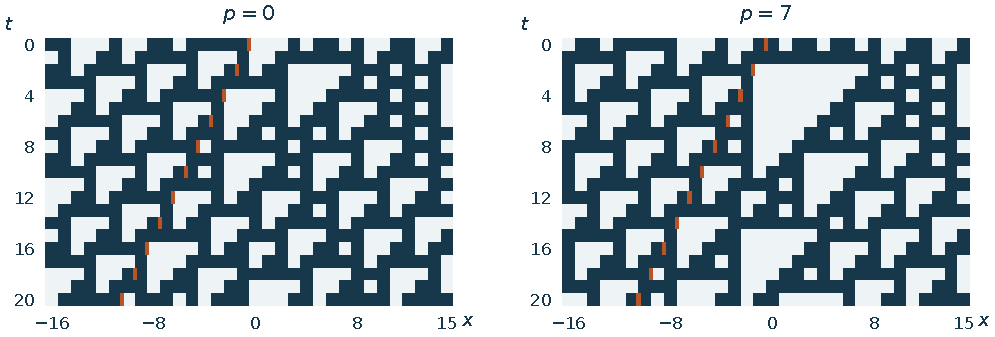
\includegraphics[width=.93\linewidth]{figures/crystal-phases.pdf}
\caption{Two phases with a common tail. For $x\ge4$, the tail is the parity of
the number of ones in the binary expansion of $x-4$. A dark cell has value 1.
The marks indicate the boundary $x=-j$ at even times. The theorem describes
the cells strictly to the left of the mark.}
\label{fig:crystal}
\end{figure}

Set $a=-j$. The automaton state stores $2j\bmod7$, $(a+p)\bmod14$, and four
bits on $[a,a+3]$. The four cells immediately to the left are given by the
crystal. Together with the window and the single new bit at $a+4$, they form
nine cells. In two steps these produce cell $a-2$ and the four bits of the new
window $[a-1,a+2]$. For all 63 reachable states, both values of the new bit
produce the correct crystal bit and an admissible successor. Ordinary locality
suffices farther to the left. These 126 checks therefore close the induction
on the entire half-line.

The two phases differ in at least one residue class modulo 14 on every time
slice. A representative can be chosen in $[-j-14,-j-1]$. Locality alone gives
the region $x<4-2j$. For $j>4$, the theorem adds $j-4$ cells to it.

\Needspace{6\baselineskip}
The asymmetry is already visible in a seven-bit window over three steps. The
leftmost input may be flipped freely, while the rightmost can be essential.
For Rule 90, both endpoints are essential. Rule 124 interchanges the two sides.
At the initial node with new bit 0, it produces 0 at the seam output instead of
the required 1. This is a concrete orientation check for the certificate.
Optimality of the boundary speed remains a separate question.

\section{When decoding needs both bits}

Place the initial bit $Y=y$ at the origin. In each context $k\in\{0,1\}$, fix
the entire remaining configuration. Denote the history by $u_{k,y}$. At time
$T$, the configurations $F^Tu_{k,0}$ and $F^Tu_{k,1}$ must agree on the whole
line for each $k$. The bit $K=k$ is read at one fixed cell of that common
configuration. The sensor takes one raw reading
$Z=(F^\tau u_{k,y})(s)$ at the same position $s$ and the same time $\tau<T$ in
all four histories.

An exact decoder receives $(K,Z)$ and returns $Y$ on all four inputs. Call both
arguments necessary if neither one alone suffices. Necessity of $K$ here means
that $Z$ alone does not suffice. Necessity of $Z$ is automatic, since both
values of $y$ occur at each fixed $k$.

\begin{theorem}\label{thm:threshold}
In this class of observations, the least time $T$ of complete coalescence is 4.
\end{theorem}

\noindent\textbf{Lower bound.}
Write $g[y]$ for the configuration obtained by setting cell 0 to $y$ in an
environment $g$. After three steps, differences between $F^3g[0]$ and
$F^3g[1]$ can occur only on $[-3,3]$. Computing these seven outputs requires
only $[-6,6]$. Once the 12 surrounding bits are specified, the central bit may
be substituted in both ways. Complete coalescence on the line is equivalent to
the window $[-6,6]$, read from left to right, having the form
\[
 \texttt{*10111[Y]1000**}.
\]
Nine positions are fixed. The three stars at positions $-6$, 5, and 6 are
free. This gives exactly eight of the 4096 environments in the window, each
with an arbitrary continuation outside it.

If two pairs coalesce by the third step, their initial configurations agree on
$[-4,4]$ for each fixed $y$. A sensor sensitive to $y$ at $\tau<3$ must have
$|s|\le\tau$. Its entire dependency region $[s-\tau,s+\tau]$ then lies in
$[-4,4]$. Consequently its responses to $y=0,1$ are the same in both contexts.
Sensitivity is required for exact decoding at fixed $k$. Hence $Y$ can be
recovered from $Z$ alone by inverting this common binary function, making the
context redundant.

Coalescence persists under further deterministic evolution. The argument
therefore excludes every $T\le3$. The following four configurations establish
attainment at step four. In the formalization, a shift moves their original
coordinate 5 to the origin.

\section{Four configurations and a stream of episodes}

Place the words from Section 4.3 of the monograph~\cite{observer} on $[-6,13]$
with a zero background. Here $Y=u(5)$, $Z=(F^2u)(3)$, and $K=(F^4u)(0)$.
Within each pair with the same $K$, only cell 5 changes. By step four, the pair
agrees everywhere. This can be checked on the 28 cells of $[-10,17]$, since
locality keeps the background zero outside this interval.

\begin{center}
\small
\begin{tabular}{@{}cclcc@{}}
\toprule
$K$ & $Y$ & Word on $[-6,13]$ & $Z$ & $O$ when $q=0$\\
\midrule
0 & 0 & \texttt{00000001100001000000} & 0 & 0\\
0 & 1 & \texttt{00000001100101000000} & 1 & 1\\
1 & 0 & \texttt{00010111010001000010} & 1 & 0\\
1 & 1 & \texttt{00010111010101000010} & 0 & 1\\
\bottomrule
\end{tabular}
\end{center}

\begin{figure}[ht]
\centering
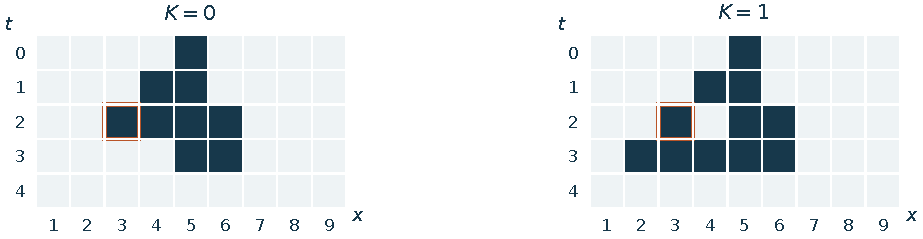
\includegraphics[width=.91\linewidth]{figures/coalescence-witnesses.pdf}
\caption{Dark cells mark coordinates where the histories with $Y=0$ and
$Y=1$ differ at a fixed $K$. The box marks the sensor at step two. There are
no differences outside the displayed region.}
\label{fig:coalescence}
\end{figure}

In the first context, $Z=Y$; in the second, $Z=1-Y$. Thus $Y=K\oplus Z$
throughout the square, whereas each individual argument takes the same value
for two different answers. This completes the proof of
Theorem~\ref{thm:threshold}. At $t=4$, cell $-2$ equals 1 in all four
configurations. Writing $Z$ into cell $-1$ and taking one step yields, at cell
$-1$, the value $f(1,Z,K)=Z\oplus K=Y$. \emph{Coalescence occurs at time 4; return occurs at
time 5.}

\begin{theorem}\label{thm:stream}
Suppose the four histories are presented according to an arbitrary external
schedule. If the register contains $q_n$ before episode $n$, writing
$q_n\oplus Z_n$ into cell $-1$ gives
\[
 q_{n+1}=q_n\oplus Z_n,\qquad O_n=q_{n+1}\oplus K_n.
\]
Before every episode $n$, we have
$q_n=q_0\oplus\bigoplus_{i<n} Z_i$. Under the same schedule, flipping $q_0$
flips every $O_n$.
\end{theorem}

The recurrence also gives $O_n=q_n\oplus Y_n$.
The proof is by induction on prefix length and applies to each index of an
infinite schedule as well. For example, episodes $(K,Y)=(0,1),(1,1)$ with
$q_0=0$ give outputs $1,0$. From the coalesced configuration alone, at fixed
$K$ and $q_0=0$, both original values of $Y$ cannot be recovered. What is
carried between episodes is the register. The schedule initializes the lattice
afresh: after the fifth step, cell $-4$ equals 1 for either injected value,
whereas that cell equals 0 in each next initial word.

\clearpage
\section{Formal proofs and reproduction}

Verification uses Lean 4.35.0. The package contains four mathematical modules
and a linking module. The file \texttt{AxiomAudit.lean} imports the canonical
seam module and prints its axiom dependencies; a separate audit imports the
ring module. The table gives the number of distinct requested reports for
each part of the proof.

\begin{center}
\footnotesize
\begin{tabular}{@{}lll@{}}
\toprule
Module & One of the checked theorems & Reports\\
\midrule
\texttt{Rule110ChiralSeam} & \texttt{counterfactual\_donor\_swap\_G5\_1} & 22\\
\texttt{Rule110RingDecoupling} & \texttt{ring7\_exact\_image\_size} & 19\\
\texttt{MergeMinimality4} & \texttt{global\_merge3\_iff\_pattern} & 11\\
\texttt{ContinuousSubject110} & \texttt{infinite\_witness\_stream} & 24\\
\texttt{MergeThreshold} & \texttt{four\_is\_least} & 3\\
\bottomrule
\end{tabular}
\end{center}

The linking module \texttt{MergeThreshold} reconciles the iteration conventions
of two files and translates the coordinates of the four words. Its theorem
\texttt{four\_is\_least} establishes both existence of the protocol at $T=4$
and the lower bound for every admissible $T$. All 79 requested axiom reports
were reproduced. They use only \texttt{propext} and \texttt{Quot.sound}.
The compiler emits four deprecation warnings for the spelling \texttt{if\_pos}
in the seam source.

From the continuation package directory, run
\texttt{python3 scripts/verify\_lean.py} to check the sources and axiom reports.
The command \texttt{python3 scripts/check\_finite.py} independently recomputes
the finite tables from the rule number. Induction supplies the unbounded time
and space claims. Run logs and checksums are included in the package.

\noindent\textbf{Publication provenance.}
The supplied Russian PDF refers to \texttt{MergeThreshold}, but that file was
absent from the supplied sources. It has been reconstructed for this
publication and checked with the four unchanged mathematical modules.
The original seam audit duplicated its implementation; the publication audit
imports it instead. A supplied historical failing log for
\texttt{MergeMinimality4} refers to a different source hash and is archived
separately; the current source compiles successfully. The reproduction paths
above have been normalized to the published directory structure.
The preparation of the text, translations, and verification code involved
assistance from ChatGPT.


\begingroup
\small
\begin{thebibliography}{9}
\bibitem{fronts}
A. Strand.
\emph{Exact Dependency Fronts, Finite Certificates, and Constructive Invariants
for Unbounded Time in Rule 110}. 2026.
Final preprint, revision \texttt{ab151b7}.
\href{https://github.com/Dnarts/rule110-dependency-fronts}{Series repository}.

\bibitem{observer}
A. Strand. \emph{110 OBSERVER: Observability of a System's Own Past}.
2026. Section 4.3. Monograph, edition 2.2.1, revision \texttt{09675a2}.
\href{https://github.com/Dnarts/rule110-dependency-fronts/tree/v2.2.1-monograph-multilingual}{Tagged source snapshot}.

\bibitem{gliders}
G. J. Mart\'inez, H. V. McIntosh, J. C. Seck-Tuoh-Mora.
\emph{Gliders in Rule 110}. International Journal of Unconventional Computing
2(1), 1--49, 2006.
\href{https://www.uaeh.edu.mx/investigacion/productos/5189/}{Authors' page}.
\end{thebibliography}
\endgroup
\end{document}
